%%%%%%%%%%%%%%%%%%%%%%%%%%%%%%%%%%%%%%%%%%%%%%%%%%%%%%%%%%%%%%%%%%%%%%%%%%%%%%%%%%%%%%%%%%%%%%%
%% Description:       Programmentwurf advanced software engineering
%% Author:      Manuel Berg, m.berg@enbw.com
%%  -*- coding: utf-8 -*-
%%%%%%%%%%%%%%%%%%%%%%%%%%%%%%%%%%%%%%%%%%%%%%%%%%%%%%%%%%%%%%%%%%%%%%%%%%%%%%%%%%%%%%%%%%%%%%%

\titlespacing*{\chapter}{0pt}{-30mm}{10pt}
\titleformat{\chapter}[display]
  {\normalfont\bfseries}{}{10pt}{\Huge\thechapter.\quad}
  
\chapter{Unit Tests (8P)}
\pagestyle{scrheadings}
\clearscrheadfoot
\pagenumbering{arabic}
\setcounter{page}{5}
\ofoot[\pagemark]{\pagemark}
%\ohead[\headmark]{\headmark}
\onehalfspacing

\section{10 Unit Tests (2P)}
\emph{[Nennung von 10 Unit-Tests und Beschreibung, was getestet wird]}

\begin{table}[htbp]
\centering
    \begin{tabular}{|l|l|}
        \hline
        \textbf{Unit Test} & \textbf{Beschreibung} \\ \hline
        ~         & ~            \\ \hline
        ~         & ~            \\ \hline
        ~         & ~            \\ \hline
        ~         & ~            \\ \hline
        ~         & ~            \\ \hline
        ~         & ~            \\ \hline
        ~         & ~            \\ \hline
        ~         & ~            \\ \hline
        ~         & ~            \\ \hline
        ~         & ~            \\
        \hline
    \end{tabular}
    \label{Tab:unit_test_table}
    \caption{Übersicht der 10 Unit Tests}
\end{table}

\section{ATRIP: Automatic (1P)}
\emph{[Begründung/Erläuterung, wie ‘Automatic’ realisiert wurde]}

\section{ATRIP: Thorough (1P)}
\emph{[Code Coverage im Projekt analysieren und begründen]}

\section{ATRIP: Professional (1P)}
\emph{[jeweils 1 positves und negatives Beispiele zu ‘Professional’; jeweils Code-Beispiel, Analyse und
Begründung, was professionell/nicht professionell an den Beispielen ist]}

\section{Fakes und Mocks (1P)}
\emph{[Analyse und Begründung des Einsatzes von 2 Fake/Mock-Objekten; zusätzlich jeweils UML
Diagramm der Klasse]}

\newpage
\titlespacing*{\chapter}{0pt}{-30mm}{10pt}
\titleformat{\chapter}[display]
  {\normalfont\bfseries}{}{10pt}{\Huge\thechapter.\quad}
  
\chapter{Domain Driven Design (8P)}
\pagestyle{scrheadings}
\clearscrheadfoot
\pagenumbering{arabic}
\setcounter{page}{6}
\ofoot[\pagemark]{\pagemark}
%\ohead[\headmark]{\headmark}
\onehalfspacing

\section{Ubiquitous Language (2P)}
\emph{[4 Beispiele für die Ubiquitous Language; jeweils Bezeichung, Bedeutung und kurze Begründung,
warum es zur Ubiquitous Language gehört]}

\begin{figure}[htbp]
\centering
\centerline{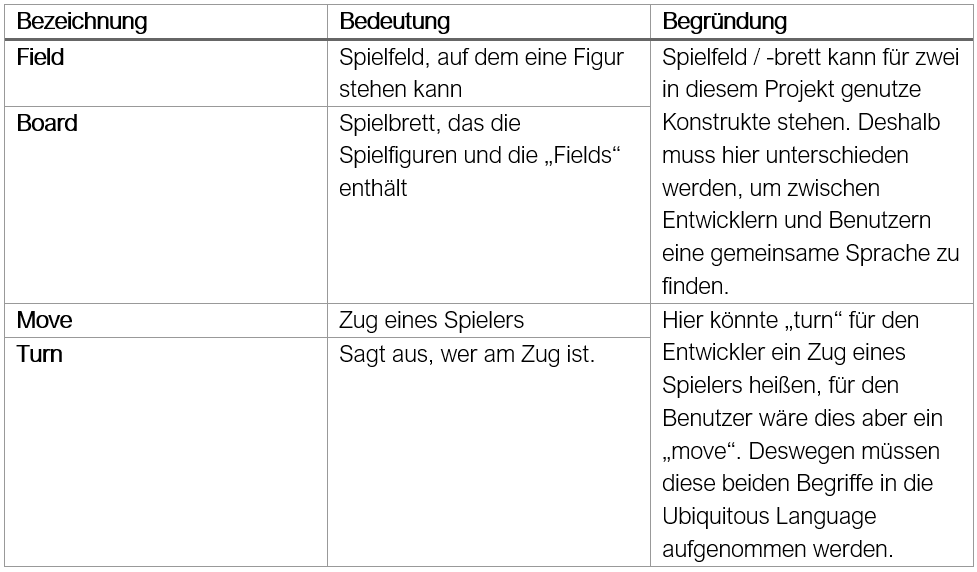
\includegraphics[scale=.7]{ubiquitous}}
\caption{4 Beispiele für die Ubiquitous Language}
\label{fig:ubiquitous}
\end{figure}

% \begin{table}[htbp]
% \centering
%     \begin{tabular}{|l|l|l|}
%         \hline
%         \textbf{Bezeichnung} & \textbf{Bedeutung} & \textbf{Begründung} \\ \hline
%         ~         & ~          & ~  \\ \hline
%         ~         & ~          & ~  \\ \hline
%         ~         & ~          & ~  \\ \hline
%         ~         & ~          & ~  \\ 

%         \hline
%     \end{tabular}
%     \label{Tab:ddd_examples}
%     \caption{4 Beispiele für die Ubiquitous Language}
% \end{table}

\section{Repositories (1,5P)}
\emph{[UML, Beschreibung und Begründung des Einsatzes eines Repositories; falls kein Repository
vorhanden: ausführliche Begründung, warum es keines geben kann/hier nicht sinnvoll ist]}

\noindent Das Repository wird durch die Klasse \enquote{GameIO} repräsentiert und bietet Zugriff auf persistenten Speicher. Außerdem wird die konkret verwendete Speichertechnologie vor dem Domain Code verborgen. In unserem Beispiel ist es das Abspeichern und Laden von Spielständen, was mithilfe von JSON umgesetzt wird. Dadurch kann ein Spiel unterbrochen und später fortgesetzt werden.

\section{Aggregates (1,5P)}
\emph{[UML, Beschreibung und Begründung des Einsatzes eines Aggregates; falls kein Aggregate
vorhanden: ausführliche Begründung, warum es keines geben kann/hier nicht sinnvoll ist]}

\begin{figure}[htbp]
\centering
\centerline{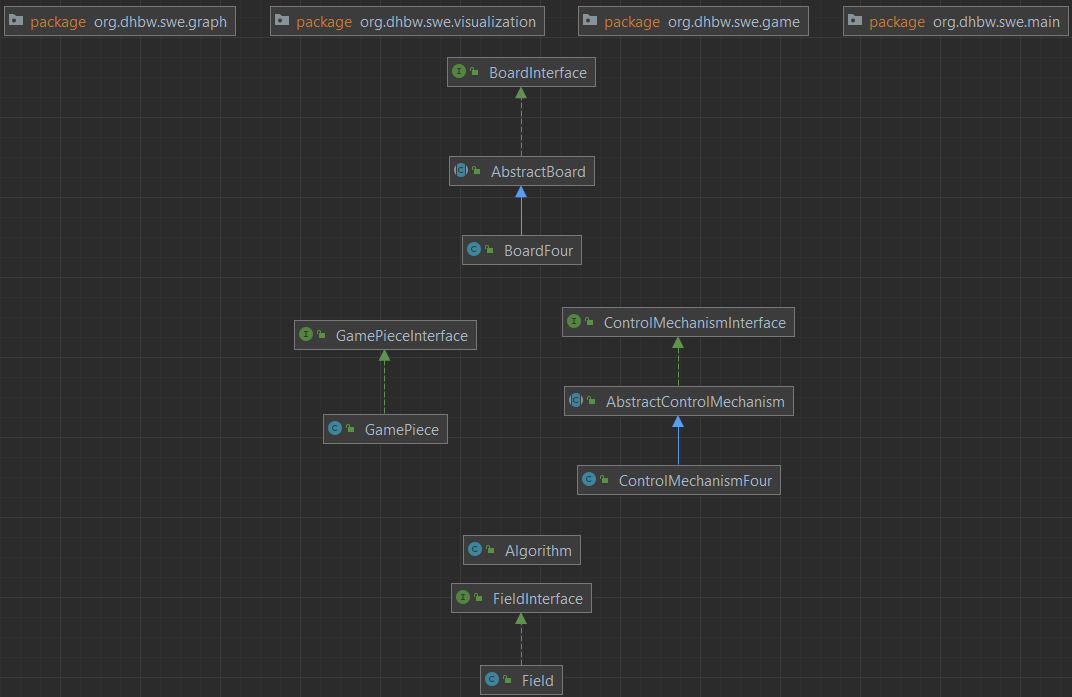
\includegraphics[scale=.6]{aggregat}}
\caption{Aggregate [Eigene Darstellung aus \emph{IntelliJ}]}
\label{fig:aggregat}
\end{figure}

\noindent Die in \hyperref[fig:aggregat]{Abbildung 6.2} dargestellten Klassen gehören zu einem Aggregat. Dies ist eine gemeinsam verwaltete Einheit und ist innerhalb seiner Grenzen konsistent. Durch diese Konsistenzgrenze war es sinnvoll, das Aggregat für das Spielbrett einzusetzen, da beispielsweise auch die Züge stets konsistent sein müssen. Als Aggregatswurzel fungiert das \enquote{BoardInterface}. Dieses kontrolliert alle Zugriffe auf das Aggregat. Wenn eines der vier oben dargestellten Packages Änderungen am Spielbrett vornehmen möchte, geht dies nur über die Aggregatswurzel. 

\section{Entities (1,5P)}
\emph{[UML, Beschreibung und Begründung des Einsatzes einer Entity; falls keine Entity vorhanden:
ausführliche Begründung, warum es keines geben kann/hier nicht sinnvoll ist]}

\noindent \textbf{ToDo: Player UUID}

\section{Value Objects (1,5P)}
\emph{[UML, Beschreibung und Begründung des Einsatzes eines Value Objects; falls kein Value Object
vorhanden: ausführliche Begründung, warum es keines geben kann/hier nicht sinnvoll ist]}

\begin{figure}[htbp]
\centering
\centerline{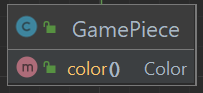
\includegraphics[scale=.6]{valueobject}}
\caption{Value Object [Eigene Darstellung aus \emph{IntelliJ}]}
\label{fig:valueobject}
\end{figure}

\noindent Ein Value Object ist hier eine Spielfigur. Diese hat als Eigenschaft nur die Farbe, welche über den gesamten Zeitraum hinweg unveränderlich bleibt. Die Änderung der Farbe ist nur durch die Konstruktion eines neuen Objektes möglich. Die Spielfigur besitzt keine eigene Identität und es ist auch kein Lebenszyklus erkennbar.

Bezüglich des \enquote{GamePiece} sind das Überschreiben von \enquote{equals()} und \enquote{hashCode()} sowie die weiteren Vorgaben aus der Vorlesung zur Implementierung von Value Objects in Java beachtet worden.

\newpage
\titlespacing*{\chapter}{0pt}{-30mm}{10pt}
\titleformat{\chapter}[display]
  {\normalfont\bfseries}{}{10pt}{\Huge\thechapter.\quad}
  
\chapter{Refactoring (8P)}
\pagestyle{scrheadings}
\clearscrheadfoot
\pagenumbering{arabic}
\setcounter{page}{7}
\ofoot[\pagemark]{\pagemark}
%\ohead[\headmark]{\headmark}
\onehalfspacing

\section{Code Smells (2P)}
\emph{[jeweils 1 Code-Beispiel zu 2 unterschiedlichen Code Smells aus der Vorlesung; jeweils Code-Beispiel
und einen möglichen Lösungsweg bzw. den genommen Lösungsweg beschreiben (inkl. (Pseudo-)Code)]}

\subsubsection{Long Method}
\noindent Dieser Code Smell war in der \enquote{calculateTurn}-Methode in der \enquote{ControlMechanismFour}-Klasse enthalten. Wie in \hyperref[fig:longmethod]{Abbildung 7.1} ersichtlich, ist die Methode viel zu lang. Zusätzlich mussten noch Kommentare eingefügt werden, dass die Methode überhaupt einigermaßen verständlich ist. 

Nach der Eliminierung des Code Smells sind nur noch die drei logischen Möglichkeiten nach den Spielregeln in der Methode enthalten. Das eigentliche Berechnen der Züge ist ausgelagert. Durch die Methodennamen sind auch keine Kommentare mehr notwendig.

\begin{figure}[htbp]
\centering
\centerline{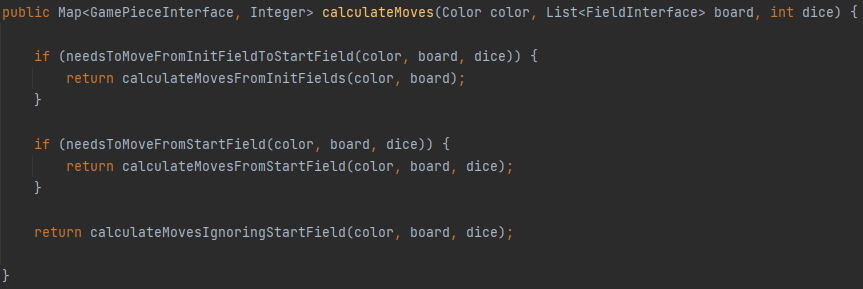
\includegraphics[scale=.5]{longmethodsolution}}
\caption{Eliminierung der Long Method [Eigene Darstellung aus \emph{IntelliJ}]}
\label{fig:longmethodsolution}
\end{figure}

\begin{figure}[htbp]
\centering
\centerline{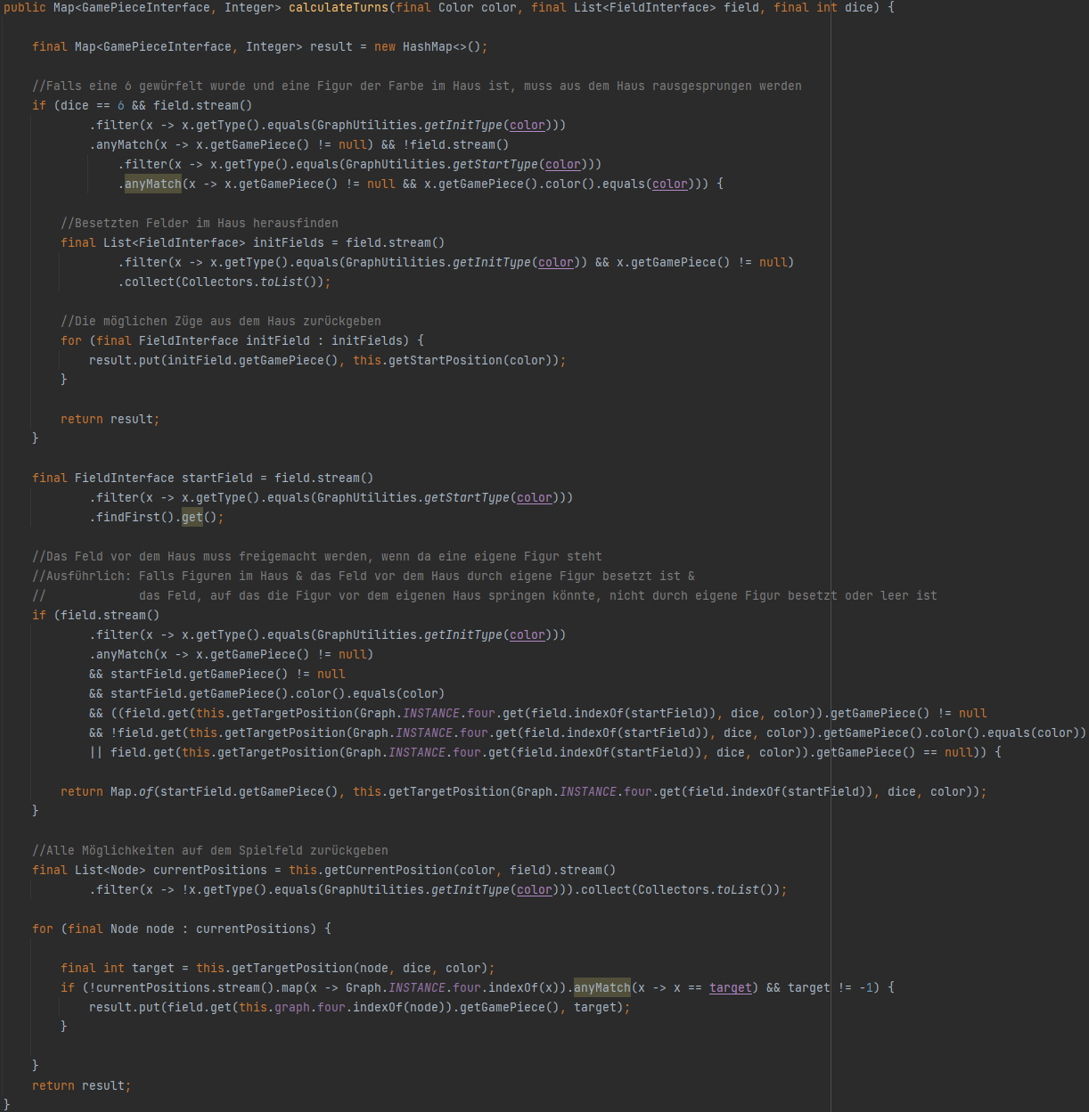
\includegraphics[scale=.65]{longmethod}}
\caption{Long Method [Eigene Darstellung aus \emph{IntelliJ}]}
\label{fig:longmethod}
\end{figure}

\newpage

\subsubsection{Switch-Statements}

\begin{figure}[htbp]
\centering
\centerline{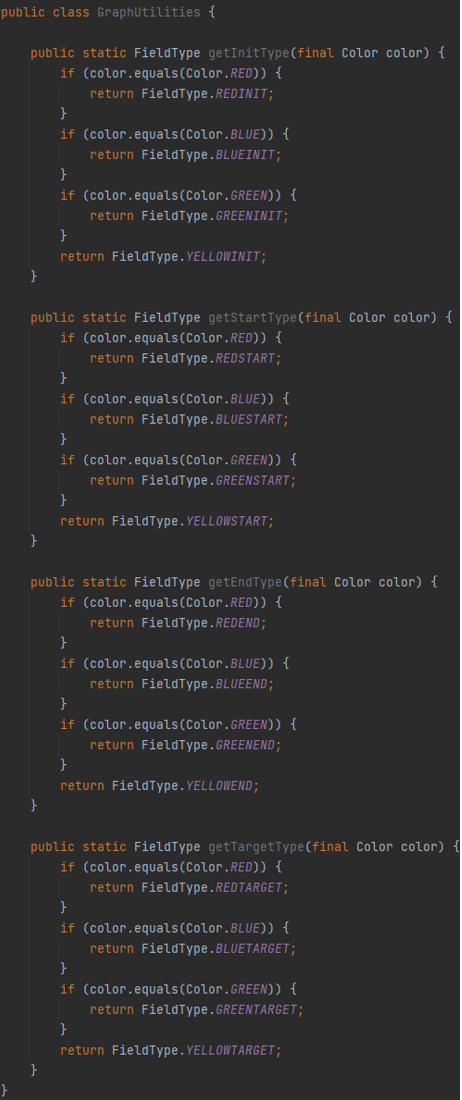
\includegraphics[scale=.55]{graphutilities}}
\caption{Switch-Statements [Eigene Darstellung aus \emph{IntelliJ}]}
\label{fig:graphutilities}
\end{figure}

\noindent Der Code-Smell bezieht sich auf die vier Methoden der \enquote{GraphUtilities}-Klasse (\hyperref[fig:graphutilities]{siehe Abbildung 7.3}). Der Switch-Statements Code Smell gilt auch hier, da die if-else-Statements einfach durch switch-Statements ersetzt werden können. Da sich diese Methoden alle um das \enquote{FieldType}-Enum drehen, wäre an dieser Stelle eine Implementierung der Methoden im Enum sinnvoller und würden den Code-Smell entfernen. 

\newpage
\noindent Das Enum wurde um fünf Instanzvariablen erweitert:

\begin{figure}[htbp]
\centering
\centerline{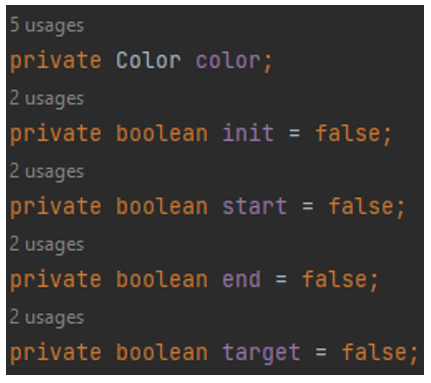
\includegraphics[scale=.55]{instanzvariablen}}
\caption{Erweiterung um fünf Instanzvariablen [Eigene Darstellung aus \emph{IntelliJ}]}
\label{fig:instanzvariablen}
\end{figure}

\noindent Außerdem wurden die vier Funktionalitäten aus den Graph-Utilities hinzugefügt:

\begin{figure}[htbp]
\centering
\centerline{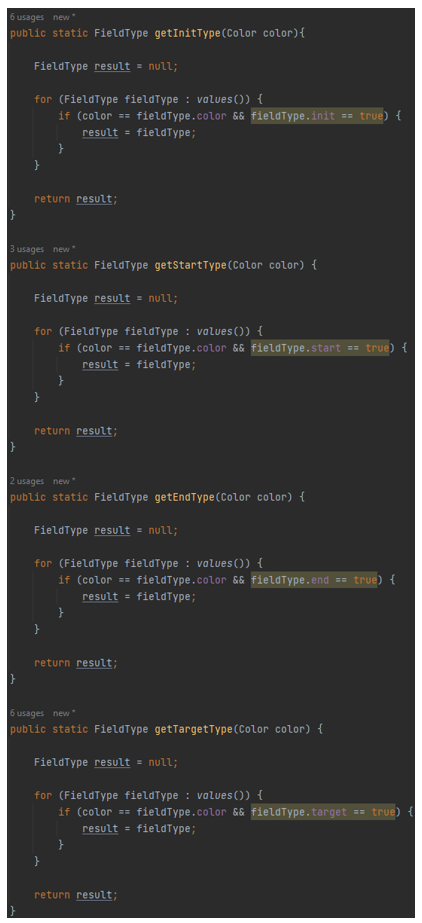
\includegraphics[scale=.8]{functionalities}}
\caption{Hinzufügen der vier Funktionalitäten [Eigene Darstellung aus \emph{IntelliJ}]}
\label{fig:funtionalities}
\end{figure}

\newpage
\section{2 Refactorings (6P)}
\emph{[2 unterschiedliche Refactorings aus der Vorlesung anwenden, begründen, sowie UML vorher/nachher
liefern; jeweils auf die Commits verweisen]}

\subsubsection{Extract Method}
\noindent Die Methode \enquote{saveGame} in der Klasse \enquote{GameIO} hat zuerst einen JSON-String erstellt und dann diesen mit dem aktuellen Zeitpunkt im Dateinamen abgespeichert. Beim Refactoring wurde hier einmal das Erstellen des JSON-Strings und das Generieren des aktuellen Zeitpunkts ausgelagert. Jetzt befindet sich nur noch der tatsächliche Abspeicherungsprozess in der Methode.

\begin{figure}[htbp]
\centering
\centerline{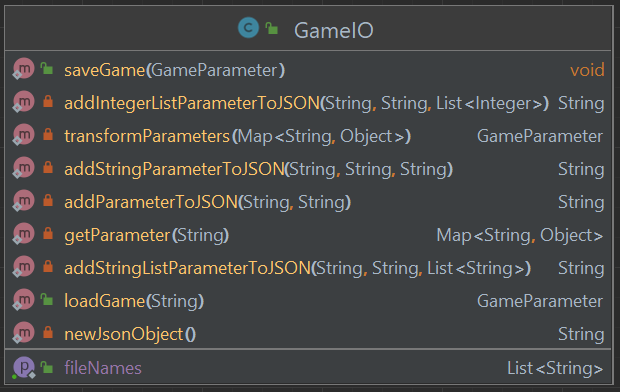
\includegraphics[scale=.5]{gameio1}}
\caption{Extract Method (vorher) [Eigene Darstellung aus \emph{IntelliJ}]}
\label{fig:gameio1}
\end{figure}

\newpage
\titlespacing*{\chapter}{0pt}{-30mm}{10pt}
\titleformat{\chapter}[display]
  {\normalfont\bfseries}{}{10pt}{\Huge\thechapter.\quad}
  
\chapter{Entwurfsmuster (8P)}
\pagestyle{scrheadings}
\clearscrheadfoot
\pagenumbering{arabic}
\setcounter{page}{8}
\ofoot[\pagemark]{\pagemark}
%\ohead[\headmark]{\headmark}
\onehalfspacing

\emph{[2 unterschiedliche Entwurfsmuster aus der Vorlesung (oder nach Absprache auch andere) jeweils
sinnvoll einsetzen, begründen und UML-Diagramm]}

\subsubsection{Entwurfsmuster: [Name] (4P)}
\subsubsection{Entwurfsmuster: [Name] (4P)}

\newpage
\titlespacing*{\chapter}{0pt}{-30mm}{10pt}
\titleformat{\chapter}[display]
  {\normalfont\bfseries}{}{10pt}{\Huge\thechapter.\quad}
  
% \chapter{Fragen an M. Müller}
% \pagestyle{scrheadings}
% \clearscrheadfoot
% \pagenumbering{arabic}
% \setcounter{page}{9}
% \ofoot[\pagemark]{\pagemark}
% %\ohead[\headmark]{\headmark}
% \onehalfspacing

% Fragen: 

% \begin{itemize}
%     %\item Dürfen wir \enquote{wir} in diesem Dokument verwenden?
%     %\item Wie genau soll die eigene Erklärung der Clean Architecture sein?
%     \item Siehe Kapitel SOLID / SRP: Ist es ok, dass wir die Klasse ControlMechanismFour nach refactoring nicht mehr haben?
%     \item Kapitel 3.2 OCP: Formulierung \enquote{Problem}
%     \item Kapitel 4.1 GRASP: Meint er mit negativ Beispiel einer geringen Kopplung eine starke Kopplung? 
%     \item Und soll die Kopplung in beiden fällen komplett aufgelöst werden oder nur zu einer geringen Kopplung gemacht werden?
%     \item Verstehen wir das richtig, dass man im DDD nur ein Repository haben kann, wenn man einen persistenten Speicher hat?
% \end{itemize}